\documentclass[conference]{IEEEtran}
\usepackage{times}

% numbers option provides compact numerical references in the text. 
\usepackage[numbers]{natbib}
\usepackage{multicol}
\usepackage[bookmarks=true]{hyperref}
\usepackage{amsmath}
\usepackage{amssymb}
\usepackage{graphicx}
\usepackage[table]{xcolor}
\usepackage{multirow}
\usepackage{color}  % For Highlighting

% Editing tools
\newcounter{RamCount}
\newcounter{DavidCount}
\newcommand{\hilight}[1]{\colorbox{yellow}{#1}}
\newcommand{\David}[1]{\textcolor{red}{\textbf{\theDavidCount}: (#1)} \addtocounter{DavidCount}{1}}
\newcommand{\Ram}[1]{\textcolor{blue}{\textbf{\theRamCount}: (#1)} \addtocounter{RamCount}{1}}
\newcommand{\Dan}[1]{\textcolor{magenta}{(#1)}}
\newcommand{\Audrey}[1]{\textcolor{maroon}{(#1)}}

%% Custom macros
\newcommand{\Real}{\mathbb{R}}

\pdfinfo{
   /Author (Daniel Bruder)
   /Title  (Modeling and Control of Soft Robots using the Koopman Operator and Model Predictive Control)
   /CreationDate (D:20101201120000)
   /Subject (Robots)
   /Keywords (Soft Robots; Koopman Operator; Model Predictive Control)
}

\begin{document}

% paper title
\title{Modeling and Control of Soft Robots using the Koopman Operator and Model Predictive Control}

% You will get a Paper-ID when submitting a pdf file to the conference system
\author{Author Names Omitted for Anonymous Review. Paper-ID [add your ID here]}

%\author{\authorblockN{Daniel Bruder}
%\authorblockA{Department of Mechanical Engineering\\
%University of Michigan\\
%Ann Arbor, Michigan 48109\\
%Email: bruderd@umich.edu}
%\and
%\authorblockN{Homer Simpson}
%\authorblockA{Twentieth Century Fox\\
%Springfield, USA\\
%Email: homer@thesimpsons.com}
%\and
%\authorblockN{James Kirk\\ and Montgomery Scott}
%\authorblockA{Starfleet Academy\\
%San Francisco, California 96678-2391\\
%Telephone: (800) 555--1212\\
%Fax: (888) 555--1212}}


% avoiding spaces at the end of the author lines is not a problem with
% conference papers because we don't use \thanks or \IEEEmembership


% for over three affiliations, or if they all won't fit within the width
% of the page, use this alternative format:
% 
%\author{\authorblockN{Michael Shell\authorrefmark{1},
%Homer Simpson\authorrefmark{2},
%James Kirk\authorrefmark{3}, 
%Montgomery Scott\authorrefmark{3} and
%Eldon Tyrell\authorrefmark{4}}
%\authorblockA{\authorrefmark{1}School of Electrical and Computer Engineering\\
%Georgia Institute of Technology,
%Atlanta, Georgia 30332--0250\\ Email: mshell@ece.gatech.edu}
%\authorblockA{\authorrefmark{2}Twentieth Century Fox, Springfield, USA\\
%Email: homer@thesimpsons.com}
%\authorblockA{\authorrefmark{3}Starfleet Academy, San Francisco, California 96678-2391\\
%Telephone: (800) 555--1212, Fax: (888) 555--1212}
%\authorblockA{\authorrefmark{4}Tyrell Inc., 123 Replicant Street, Los Angeles, California 90210--4321}}


\maketitle

\begin{abstract}
%% Robots are hard to control
Controlling soft robots with precision is a challenge due in large part to the difficulty of constructing models that are amenable to model-based control design techniques.
%% Koopman operator their offers a solution
Koopman Operator Theory offers a way to construct explicit linear dynamical models of soft robots and to control them using established model-based linear control methods.
This method is data-driven, yet unlike other data-driven models such as neural networks, it yields an explicit control-oriented linear model rather than just a ``black-box'' input-output mapping.
%% Summary of contributions
This work describes this Koopman-based system identification method and its application to model predictive controller design.
%% Experiment and results
A model and MPC controller of a pneumatic soft robot arm was constructed via the method, and its performance was evaluated over several trajectory following tasks in the real-world. 
On all of the tasks, the Koopman-based MPC controller outperformed a benchmark MPC controller based on a linear state-space model of the same system.
\end{abstract}

\IEEEpeerreviewmaketitle

%% Insert all content here
\section{Introduction} 
\label{sec:intro}

%% Why soft robots?
%% Body softness has been shown to be useful for robots operating in unstructured/unpredictable environments, or alongside humans, but hard to control.
Soft robots have bodies made out of intrinsically soft and/or compliant materials.
This inherent softness enables them to safely interact with delicate objects, and to passively adapt their shape to unstructured environments \cite{rus2015design}.
Such traits are desirable for robotic applications that demand safe human-robot interaction such as wearable robots, in-home assistive robots, and medical robots.
Unfortunately, the soft bodies of these robots also impose modeling and control challenges, which have restricted their functionality to date. 
In fact, many novel soft devices such as soft grippers (cite), crawlers (cite), and swimmers (cite) exploit the flexibility of their bodies to achieve coarse behaviors such as grasping and locomotion, but do not exhibit precise control capabilities \Dan{don't forget to add citations here}.
% Emulating the functionality of the dexterous and precise soft systems found in nature such as octopus arms, elephant trunks, and tongues stems from the inherent difficulty of modeling continuum structures and controlling nonlinear dynamical systems.

% Unfortunately, their soft bodies also make soft robots notoriously difficult to model and control, limiting their functionality to date. 
% While their compliance enables such behavior it also makes soft robots challenging to model and control \cite{rus2015design}.

% Soft systems found in nature such as octopus arms, elephant trunks, and tongues display incredible dexterity and precision \cite{vogel2000cats}, but such functionality has yet to be realized in soft robots.
% Many novel devices such as soft grippers (cite), crawlers (cite), and swimmers (cite) exploit the flexibility of their bodies to achieve coarse behaviors such as grasping and locomotion, but do not exhibit precise control capabilities
% can be attributed to two innate characteristics of soft systems: continuum structure, and nonlinear dynamical behavior. 


%% Technical challenges to modeling: continuum structure
% Even building models for soft robots presents a challenge.
The challenge in constructing such precise control techniques is due in large part to the difficulty of devising models of soft robots that are amenable to model based control design techniques.
% Mathematical models are a convenient tool for predicting behavior and designing controllers for robots, but useful models are not as readily available for soft robots as for rigid-bodied ones \Ram{citation?}.
Consider for instance rigid-bodied robotic systems that are made up of rigid links connected together by discrete joints.
% Rigid-bodied robots consist of rigid links connected together by discrete joints.
%It has been shown that the full geometry of a rigid-bodied system can be described in terms of joint deformations, making joint deformations the canonical choice of state variables for rigid-bodied robots \cite{spong2008robot}.  %[Brent thinks the following would be a little easier to read:]
Since joint displacements can be used to fully describe the configuration of a rigid-bodied system, joint displacements and their derivatives make a natural choice for the state variables for rigid-bodied robots \cite{spong2008robot}.
One can use this choice of state variables to describe the dynamics of the rigid-bodied robot.
This, as a result, makes the application of model-based control design techniques such as feedback linearization \cite{}, nonlinear model predictive control \cite{}, LQR-trees \cite{}, sequential action control \cite{ansari2016sequential}, and others feasible. \Dan{don't forget to add citations here} 

Soft robots, in contrast, do not exhibit localized deformation at discrete joints, but instead deform continuously along their bodies and have infinite degrees-of-freedom.
In the absence of joints, there does not yet exist a canonical choice of state variables to describe the geometry of a soft robot.
% Instead, it is common practice to choose a state made up of observable parameters, such as end-effector position (cite our koopman paper), curvature of body (cite), or fluid pressure (cite) \Dan{think of better example(s)}.
As a result, existing representations are typically only rich enough to describe the system under restrictive simplifying assumptions.
For example, the popular piecewise constant curvature model \cite{webster2010design} provides a low-dimensional description of the shape of continuum robots, but only under the assumption that bending occurs in sections of constant curvature.
Other simplified models such as pseudo-rigid-body (cite) and quasi-static \cite{bruder2018iros} (cite others), have demonstrated sufficient accuracy for some objectives (cite), \Dan{don't forget to add citations here} 
but they are only able to describe the behavior in a subset of configurations of the soft robot which can make applying model-based control design techniques impractical. 

%% FIGURE: Overview of the different system representations and control approaches
\begin{figure}
    \centering
    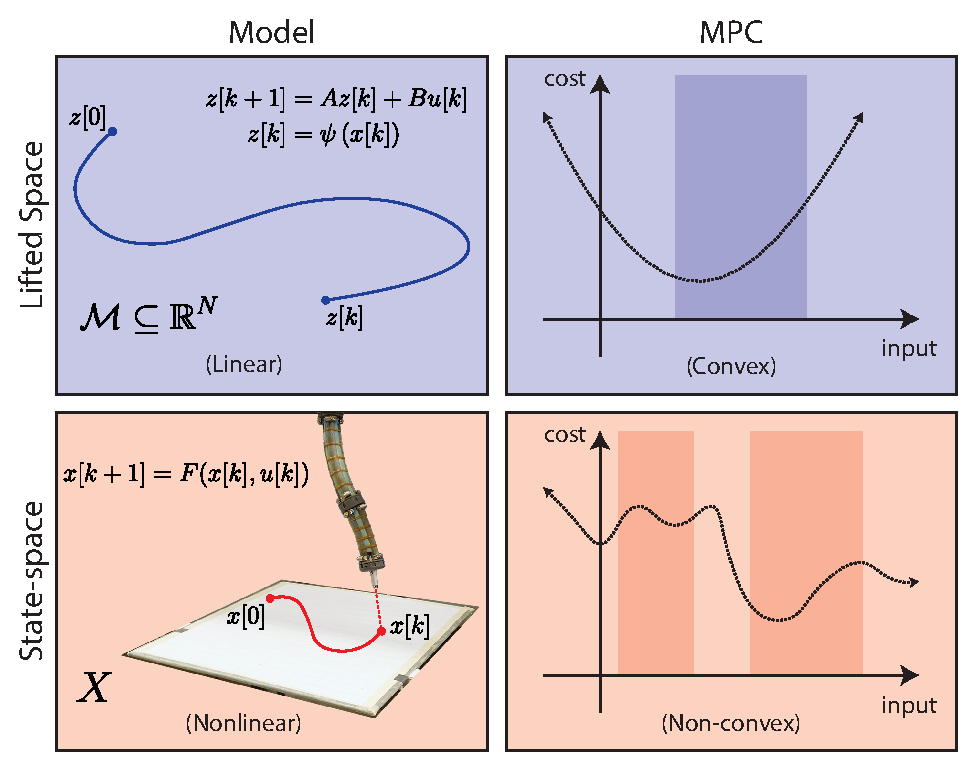
\includegraphics[width=\linewidth]{figures/overview_v8.pdf}
    \caption{A nonlinear dynamical system (bottom-left) has a \emph{linear} representation in the \emph{lifted} space made up of all real-valued functions (top-left). While a model predictive controller (MPC) designed for the nonlinear system in state-space requires solving a non-convex optimization problem to choose inputs at each time-step (bottom-right), this problem is convex for an MPC controller designed for the lifted linear system (top-right). This paper develops a data driven method to construct such a lifted model representation  for soft robotic systems in the presence of outliers and a convex, model-based control design technique for such systems. }
    \vspace*{-0.5cm}
    \label{fig:overview}
\end{figure}

%% data-driven models: don't make assumptions but not great for building controllers
% \Dan{This paragraph is a mess. Going to step away and come back to it}
Alternatively, data-driven methods, such as machine learning and neural networks, can be applied to construct models for soft robots without making structural simplifying assumptions.
Such models serve as a ``black-box'' by mapping from inputs to outputs and have been shown to predict behavior well across various configurations of the soft robot  \cite{gillespie2018learning, thuruthel2018model}.
However, since no explicit model is constructed, it can be challenging to apply existing model-based control design techniques.
% While such ``black-box'' models have been shown to predict behavior well, they offer little insight when it comes to controller design.
% \Ram{can you be more explicit here?} 

%% Technical challenge to control: Nonlinear dynamical behavior (think about this more and fix it)
% The inherently nonlinear dynamical behavior of soft robots presents a control challenge (CITE LASCHI CONTROL PAPER).
% Linear dynamical systems obey the \emph{superposition principle} (cite), which has enabled the development of powerful tools that render the task of controlling linear systems almost trivial.
% Unfortunately, the superposition principle does not hold for nonlinear dynamical systems and consequently there is no universal approach to controlling them.
% Numerical control techniques, such as nonlinear model predictive control (NMPC), have become popular due to ongoing increases in computational power and affordability.
% However, such methods require iteratively solving nonlinear non-convex optimization problems, for which global convergence is not guaranteed \cite{boyd2004convex}.
% which suffer from numerical issues such as suboptimal convergence and slow execution . 
% Numerical solvers may converge to suboptimal local extrema rather than optimal values.
% they are also slow...
% While this problem is not limited to soft robots (few mechanical systems exhibit completely linear dynamic behavior), soft robots are not as amenable to approximate linear descriptions as many other systems.

%% Koopman approach exists and can help here, it just needs some tweaks to work well for a real system
Koopman Operator Theory offers an approach that can overcome the challenges of modeling and controlling soft robots.
The Koopman operator approach is data-driven yet produces an explicit control-oriented model that is linear (though higher dimensional).
% Laid out in \citet{korda2018linear}, 
The approach leverages the linear structure of the Koopman operator to construct linear models of nonlinear controlled dynamical systems from input-output data \cite{bruder2018nonlinear, mauroy2016linear}, and to control them using established linear control methods \cite{Abraham-RSS-17, korda2018linear}.
In theory, this approach involves \emph{lifting} the state-space to an infinite-dimensional space of scalar functions (referred to as observables), where the flow of such observables along trajectories of the nonlinear dynamical system is described by the \emph{linear} Koopman operator.
In practice, however, it is not feasible to compute an infinite-dimensional operator, so a modified version of the Extended Dynamic Mode Decompostion (EDMD) is employed to compute a finite-dimensional projection of the Koopman operator onto a finite-dimensional subspace of all observables (scalar functions).
This approximation of the Koopman operator describes the evolution of the values of the output variables themselves, provided that they lie within the finite subspace of observables upon which the operator is projected.
Hence, this approach makes it possible to control the output of a nonlinear dynamical system using a linear controller designed for its linear Koopman representation.

%% Why this approach is uniquely well suited for soft robots: 
The Koopman approach to modeling and control is well suited for soft robots for several reasons.
Soft robots pose less of a physical threat to themselves or their surroundings when subjected to random control inputs than conventional rigid-bodied robots. 
This makes it possible to safely collect input-output data over a wide range of operating conditions, and to do so in an automated fashion. 
Furthermore, since the Koopman procedure is entirely data-driven, it inherently captures input-output behavior and avoids the ambiguity involved in choosing a discrete set of states for a structure with infinite degrees of freedom.
% Soft robots are also nonlinear dynamical systems, but this approach generates a linear system representation.
% As will be shown later, this linear representation can be used to construct a controller which computes control inputs by solving a convex optimization problem at each time step.

%% Our contribution: Modifications/additions needed to get this to reliably work for a real system
% This work applies the Koopman based system identification method from \citet{mauroy2016linear} and the Koopman based model predictive control method from \citet{korda2018linear} to a real soft robotic system.
The work presented here can be considered an extension of the work on Koopman-based modeling and control of \citet{mauroy2016linear} and \citet{korda2018linear}.
The novel contributions of this work, as depicted in Fig. \ref{fig:overview} are:
\begin{enumerate}
    \item An extension to the Koopman system identification procedure described in \cite{mauroy2016linear} to make the resulting Koopman operator both more sparse and less sensitive to outliers and noise in the training data,
    \item The application of this identified Koopman model for model predictive control of a physical soft robotic system.
\end{enumerate}
% We achieve (1) by introducing an $L^1$ penalty term into the least-squares optimization problem used to solve for the approximate Koopman operator.
Contribution (1) arose by necessity from the pursuit of contribution (2), since real mechanical systems suffer from both noise and computational limitations. \Dan{Rewrite this last sentence.} \Ram{my suggestion is that you highlight in the previous paragraph (the one about the utility of applying Koopman operator theory to soft robots) that pressure regulators for soft robots suck so they are super noisy which can make identifying such a Koopman model in practice difficult.}
% Data collected from physical mechanical systems is prone to noise, which can lead to over-fitting of data-driven models.
% Because real mechanical systems suffer from noise this step is 
% Both of these are desirable features when working with real systems, which suffer from noise and computational limitations.



%% Outline
The rest of this paper is organized as follows:
In Section \ref{sec:sysid} we formally introduce the Koopman operator and describe how it is used to construct linear models of nonlinear dynamical systems. 
In Section \ref{sec:mpc} we describe how the Koopman model can be used to construct a linear model predictive controller.
In Section \ref{sec:experiments} we describe the soft robot and the set of experiments used to evaluate the performance of a Koopman-based MPC controller.
In Section \ref{sec:conclusion} concluding remarks and perspectives are provided.





% %% Solution: Data-driven/linear representation, description of koopman approach
% In this paper, we present a novel method for the modeling and control of soft robots based on Koopman Operator Theory.
% This method addresses the challenges of modeling and control by offering a way to build a \emph{linear} model from data that still captures the \emph{nonlinear} input-output behavior of a soft robot.
% This approach is based on the system identification method originally presented in \citet{mauroy2017koopman} and the control approach laid out in \citet{korda2018linear}.
\section{Theory}
\label{sec:theory}

%% Overview of this section
Any finite-dimensional nonlinear dynamical system has an equivalent infinite-dimensional linear representation in the space of real-valued functions of the system's state \cite{}.
In this function space, the (linear) Koopman Operator describes the flow of functions along trajectories of the system.
% The dual of the Koopman operator, the Perron-Frobenius operator, describes the dynamics of the system...
While it is not possible to fully represent the infinite-dimensional Koopman operator, it is possible to represent its projection onto a finite-dimensional subspace.


%% Overview of the Koopman operator and how it represents dynamical systems
\subsection{Koopman Representation of Dynamical Systems}

%% System representation in state space
Consider a dynamical system
\begin{align}
    \dot{x} &= F (x)    \label{eq:nlsys}
\end{align}
where $x \in \Real^n$ is the state of the system and ${F}$ is continuously differentiable in $x$.
Denote by $\phi(t,x_0)$ the solution to \eqref{eq:nlsys} at time $t$ when beginning with the initial condition $x_0$ at time $0$.
For simplicity, we denote this map, which is referred to as the \emph{flow map}, by $\phi^t (x_0)$ instead of $\phi (t, x_0)$.

%% System representation in the space of observables
The system can be lifted to an infinite dimensional function space $\mathcal{F} = L^2(X, \Real)$ where $X \subset \Real^n$ is a compact subset and $L^2(X , \Real)$ is the space of square integrable real-valued functions with domain $X$.
Elements of $\mathcal{F}$ are called \emph{observables}.
In $\mathcal{F}$, the flow of the system is characterized by the set %semigroup 
of Koopman operators 
$U^t : \mathcal{F} \to \mathcal{F}$, for each $t \geq 0$,
which describes the evolution of the observables ${f \in \mathcal{F}}$ along the trajectories of the system according to the following definition:
\begin{align}
    U^t f = f \circ \phi^t      
    % && \forall f \in \F, t \geq 0
    \label{eq:koopman}
\end{align}
As desired, $U^t$ is a linear operator even if the system \eqref{eq:nlsys} is nonlinear, since for $f_1, f_2 \in \mathcal{F}$ and $\lambda_1, \lambda_2 \in \Real$
\begin{align}
    \begin{split}
    U^t (\lambda_1 f_1 + \lambda_2 f_2) &= \lambda_1 f_1 \circ \phi^t + \lambda_2 f_2 \circ \phi^t \\
    &= \lambda_1 U^t f_1 + \lambda_2 U^t f_2.
    \end{split}
\end{align}
Thus the Koopman operator provides a linear representation of the flow of a nonlinear system in the infinite-dimensional space of observables (see Fig. \ref{fig:overview}) \cite{budivsic2012applied}.


%% Koopman-based system identification (consult ICRA paper)
\subsection{Identification of Koopman Operator}

Since the Koopman operator is an infinite-dimensional object, it cannot be represented by a finite-dimensional matrix. 
Therefore, we settle for the projection of the Koopman operator onto a finite-dimensional subspace.
Using the system identification method originally presented in \cite{mauroy2016linear} and \cite{mauroy2017koopman}, we identify a finite-dimensional approximation of the Koopman operator via linear regression performed on observed data.

Define ${\bar{\mathcal{F}} \subset \mathcal{F}}$ to be the subspace of $\mathcal{F}$ spanned by $N$ linearly independent basis functions $\{ \psi_k \}_{k=1}^N$.
Any observable $\bar{f} \in \bar{\mathcal{F}}$ can be expressed as a linear combination of elements of these basis functions
\begin{align}
    \bar{f} &= \alpha_1 \psi_1 + \cdots + \alpha_N \psi_N
\end{align}
where each $\alpha_i \in \Real$.
For notation, we introduce the vector of coefficients ${\alpha = [ \alpha_1 \,  \cdots \, \alpha_N ]^T}$ and the \emph{lifting function} $\psi : \Real^n \to \Real^N$ defined as:
\begin{align}
    \psi(x) &:= \begin{bmatrix} \psi_1 (x) & \cdots & \psi_N (x) \end{bmatrix}^T.
    \label{eq:lift}
\end{align}
Then, $\bar{f} \in \bar{\mathcal{F}}$ can be expressed concisely as
\begin{align}
    \bar{f} &= \alpha^T \psi
    \label{eq:fvec}
\end{align}
Via \ref{eq:fvec}, $\alpha$ provides a vector representation for $\bar{f} \in \bar{\mathcal{F}}$.

Given this vector representation for observables, a finite-dimensional approximation of the Koopman Operator can be represented by a matrix.
We denote by $\bar{U}^t \in \Real^{N \times N}$ the approximation of the Koopman Operator in $\bar{\mathcal{F}}$, which operates on observabels via matrix multiplication:
\begin{align}
    \bar{U}^t \alpha = \beta
\end{align}
where $\alpha , \beta$ are each vector representations of observables in $\bar{\mathcal{F}}$.
%% Pulled straight from ICRA paper below this line
Our goal is to find a $\bar{U}^t$ that describes the action of the infinite dimensional Koopman operator $U^t$ as accurately as possible in the $L^2$-norm sense on the finite dimensional subspace $\bar{\mathcal{F}}$  of all observables.
Therefore, to perfectly mimic the action of $U^t$ acting on an observable in $\bar{\mathcal{F}} \subset \mathcal{F}$, the following should be true
\begin{align}
    ( \bar{U}^t {\alpha} )^T {\psi}(x) &=
    {\alpha}^T {\psi} \left( \phi^t(x) \right).
    \label{eq:UbarEq}
\end{align}
Since this is a linear equation, it follows that for a given ${x \in \Real^n}$, solving \eqref{eq:UbarEq} for $\bar{U}^t$ yields the best approximation of $U^t$ on $\bar{\mathcal{F}}$ in the $L^2$-norm sense:
\begin{align}
    \bar{U}^t = \left( {\psi}(x)^T \right)^\dagger {\psi}( \phi^t(x) )^T
    \label{eq:Uapprox}
\end{align}
where superscript $\dagger$ denotes the least-squares pseudoinverse.

%% How this is done on our system
To approximate the Koopman operator from a set of experimental data, we take $K+1$ discrete state measurements with sampling period $T_s$. We separate the data into a set of $K$ so-called ``snapshot pairs'' of the form ${ \{ x_k , y_k \} \in \Real^{n \times 2} }$ where
\begin{align}
    y_{k} &= \phi^{T_s} (x_k) + \sigma_k
\end{align}
and $\sigma_k$ denotes measurement noise.
% For our basis of $\bar{\mathcal{F}}$, we choose the basis of monomials of $x$ with total degree less than or equal to $w$, which implies ${N=(n+m+w)!/\left((n+m)!w!\right)}$ \cite[Section III]{mauroy2016linear}. 
We then lift all of the snapshot pairs according to \eqref{eq:lift} and compile them into the following ${K \times N}$ matrices:
\begin{align}
    &\Psi_x = \begin{bmatrix} {\psi}(x_1)^T \\ \vdots \\  {\psi}(x_K)^T \end{bmatrix}
    &&\Psi_y = \begin{bmatrix} {\psi}(y_1)^T \\ \vdots \\  {\psi}(y_K)^T \end{bmatrix}
\end{align}
$\bar{U}^{T_s}$ is chosen so that it yields the least-squares best fit to all of the observed data, which, following from \eqref{eq:Uapprox}, is given by 
\begin{align}
    \bar{U}^{T_s} &:= \Psi_x^\dagger \Psi_y.
\end{align}

%% The Koopman MPC problem (consult Mezic paper)
\subsection{Model Predictive Control}
\section{Experiment}
\label{sec:methods}

%% Introduction
Because the Koopman model is linear, it can be used to design linear controllers for nonlinear dynamical systems.


%% Description of system
\subsection{Description of System: Soft Arm with Laser Pointer}

The soft robot system used in experiments consists of two sections composed of three pneumatically driven McKibben actuators (also known as Pneumatic Artificial muscles or PAMs) adhered to a central foam spine by latex rubber suspended from a raised platform (see Fig. \Dan{Add figure with photo and schematic of robot}) .
The PAMs in the upper and lower sections are internally connected and arranged such that they share three input pressure lines and for any bending of the upper section, there is bending in the opposite direction in the bottom section.
This ensures that the laser pointer mounted to the end effector roughly points down at all times.
Roughly 30 cm beneath the hanging arm lies a flat board where the laser dot is projected.
A digital webcam aimed at the board is used to capture the position of the laser dot during trials.

%% Rig figure
\begin{figure}
    \centering
    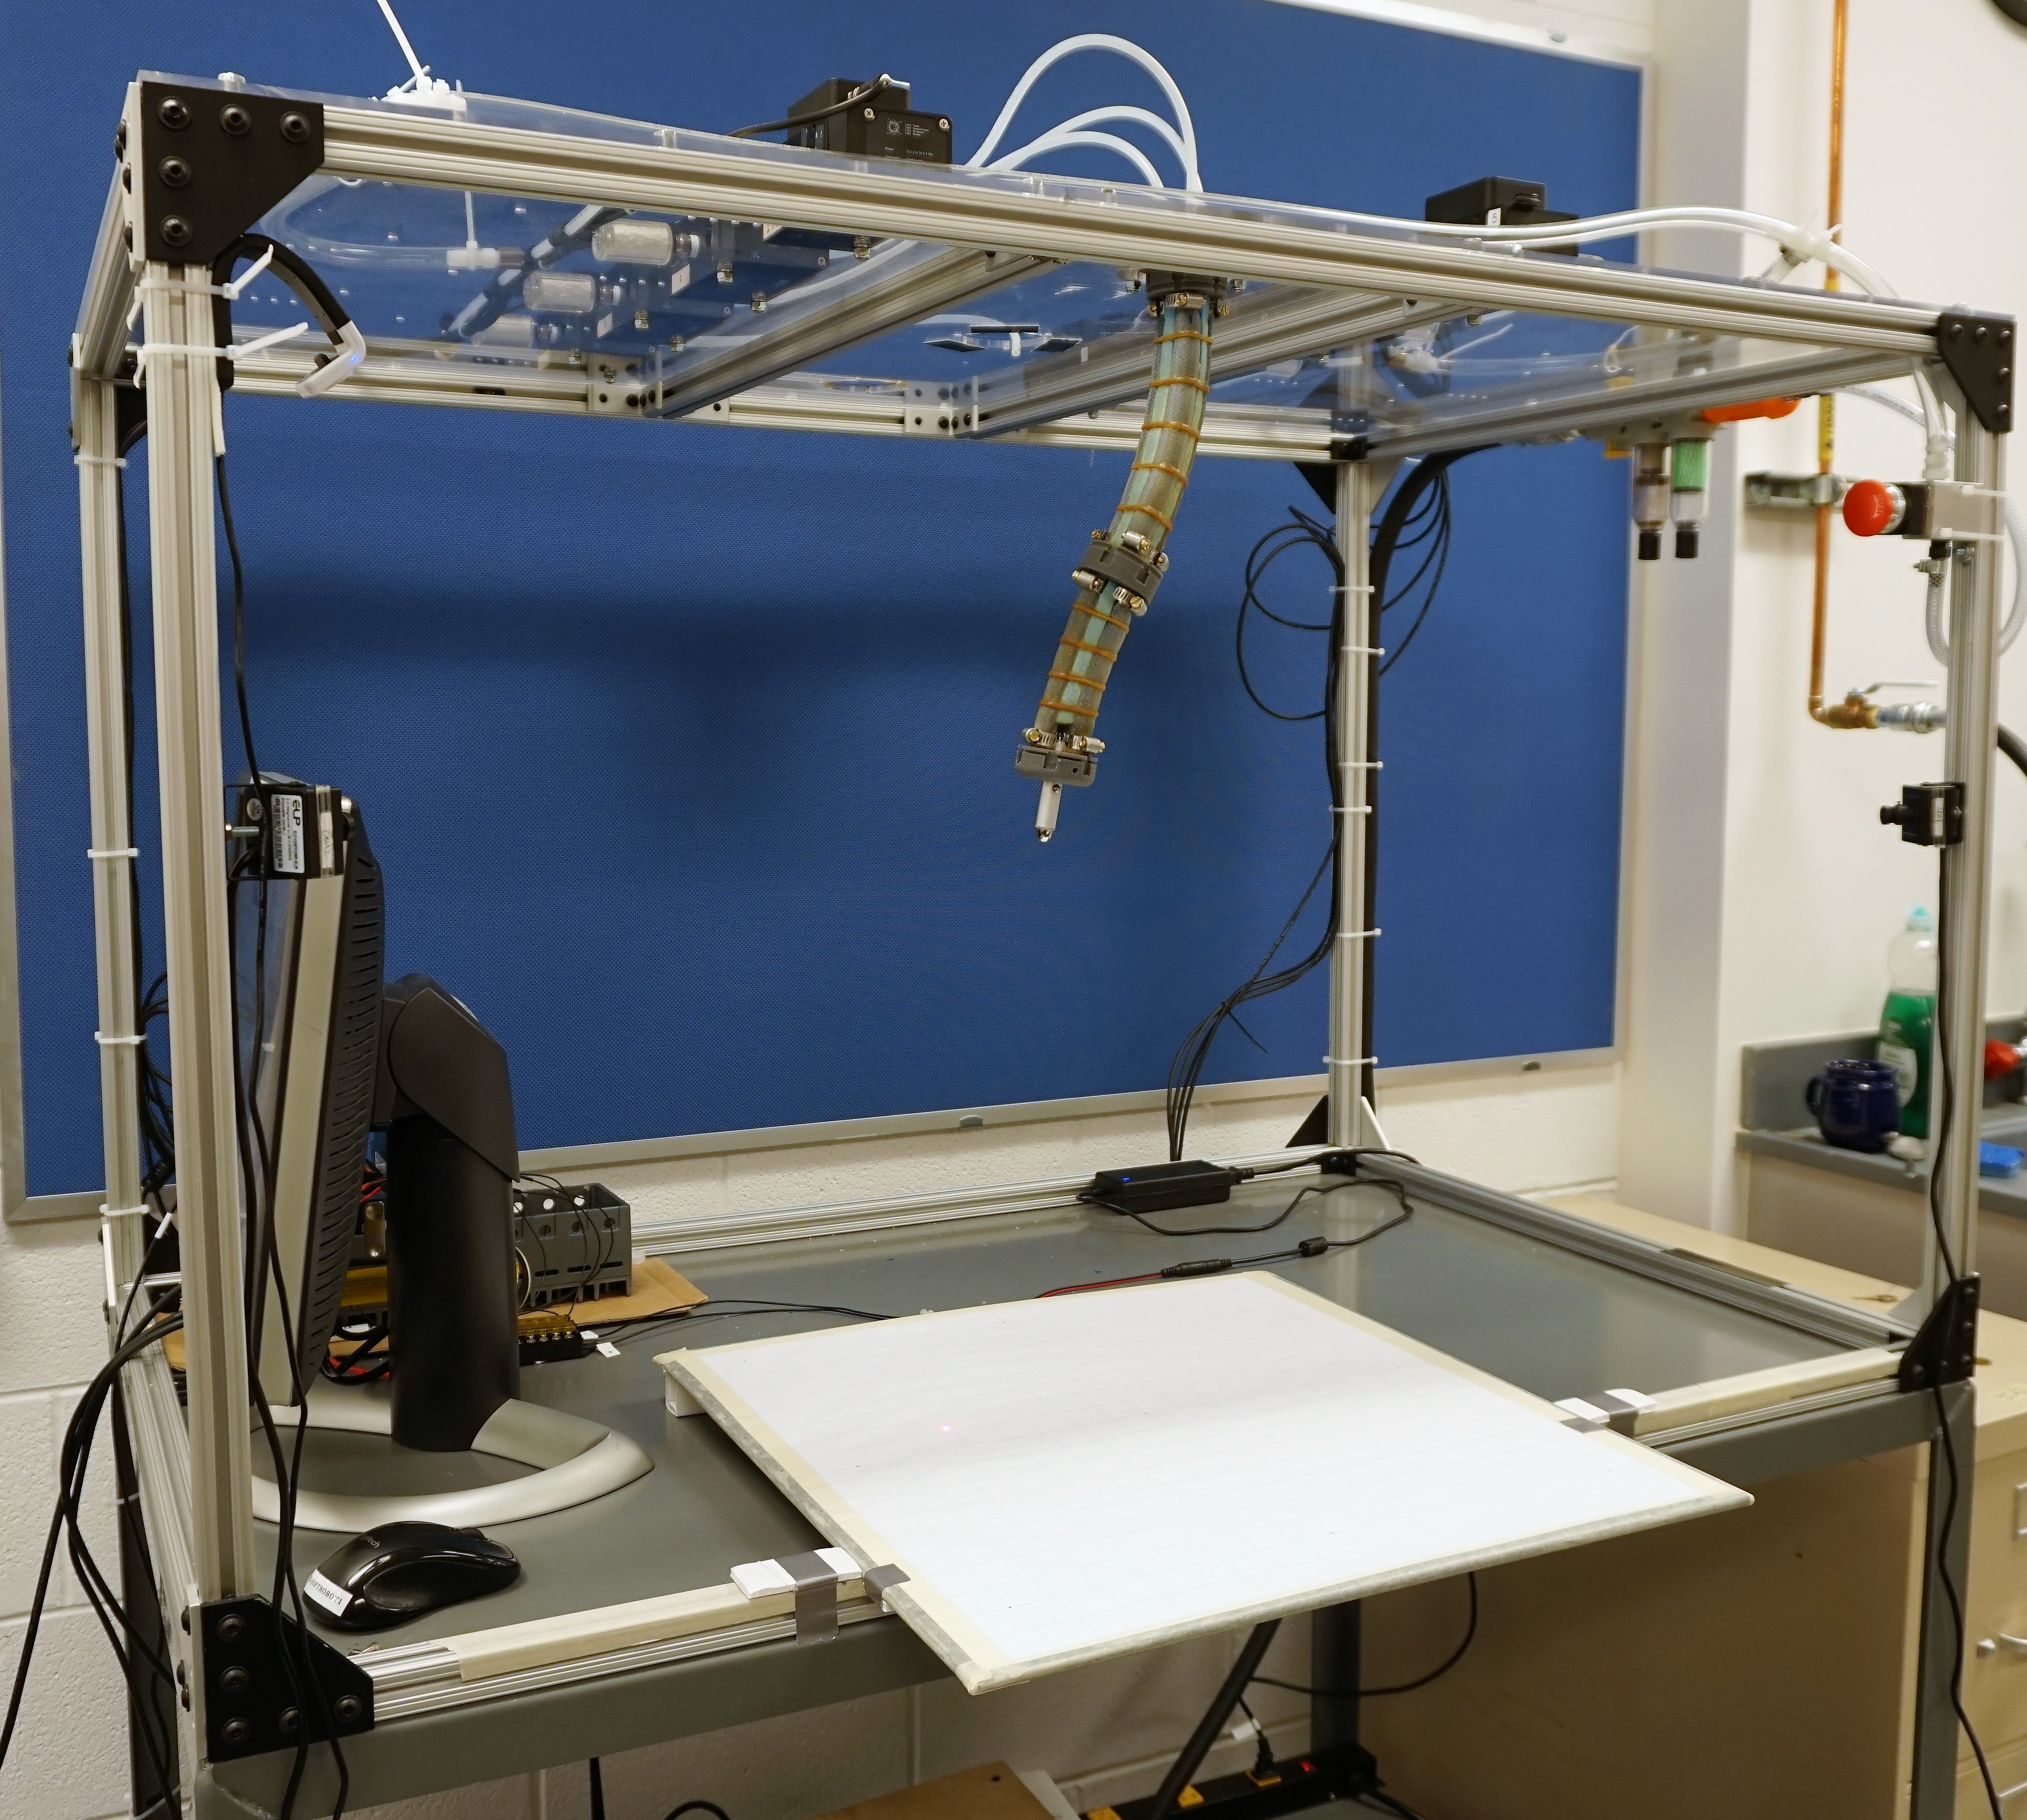
\includegraphics[width=\linewidth]{figures/DSC00707_cropped.jpg}
    \caption{\Dan{current placeholder for version with labels and possibly with background photoshopped out.}}
    \label{fig:rig}
\end{figure}

%% Robot figure
\begin{figure}
    \centering
    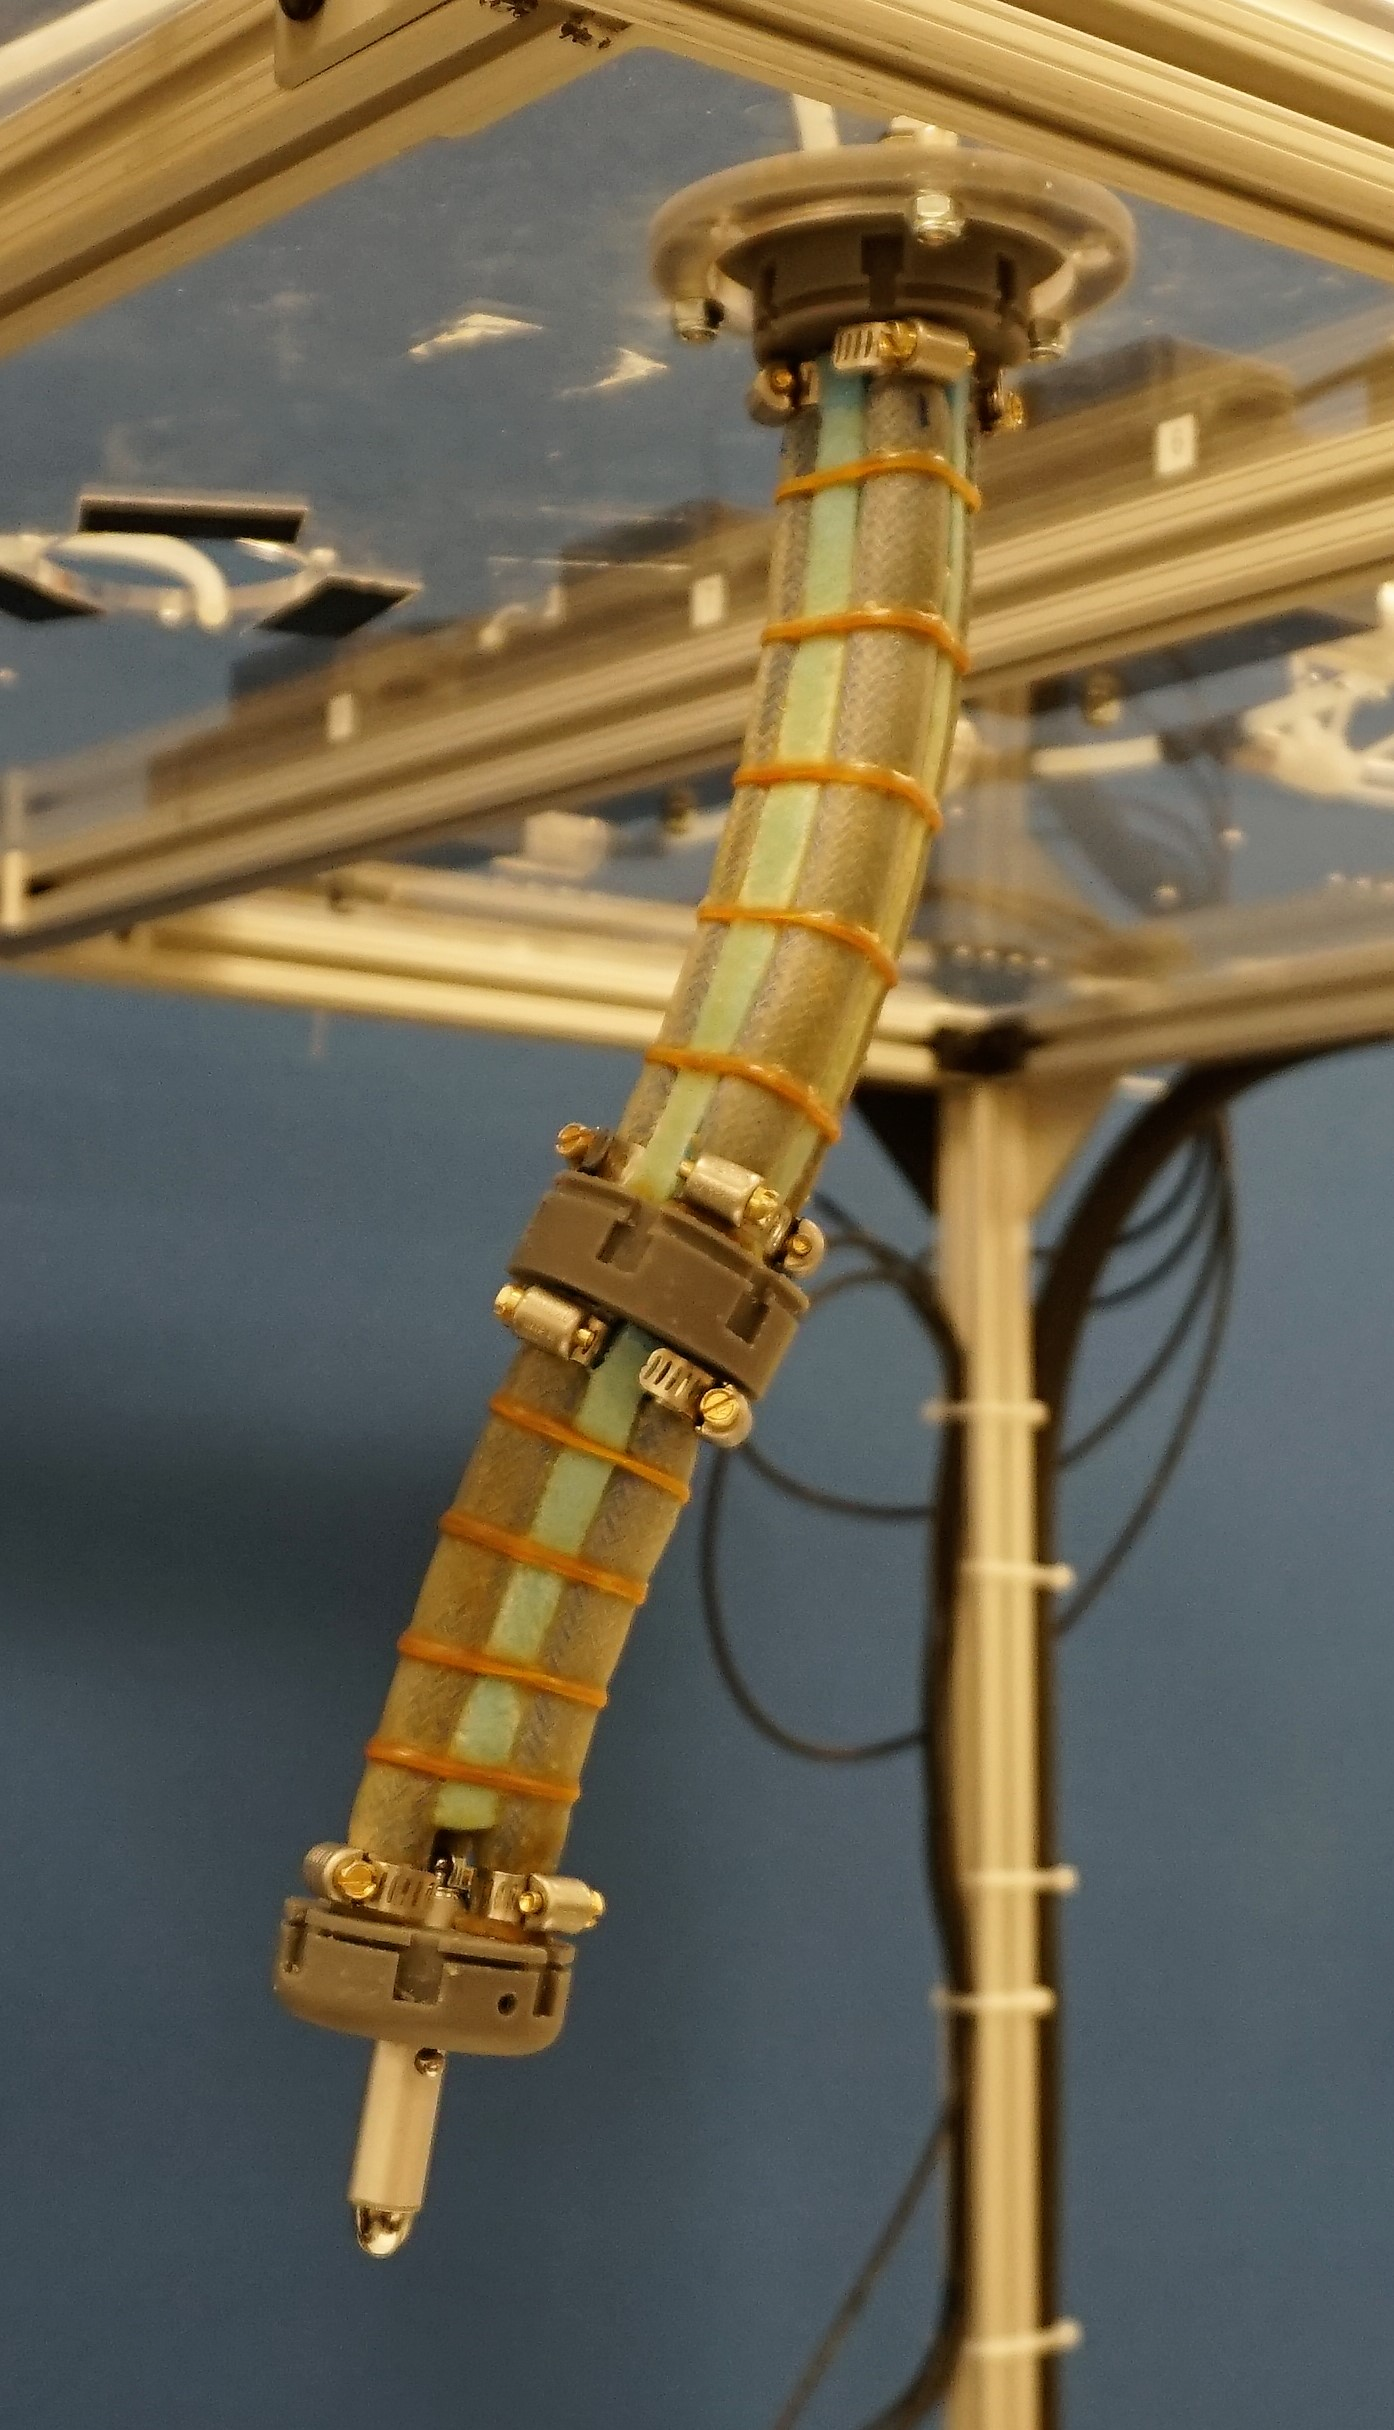
\includegraphics[width=0.5\linewidth]{figures/closeup.jpg}
    \caption{\Dan{Will also include a closeup of robot like this if space permits}}
    \label{fig:robot}
\end{figure}

%% Description of compared controllers
\subsection{Description of Controllers}

\begin{itemize}
    \item K-MPC: Koopman model predictor
    \item L-MPC: linear state-space model predictor
    \item N-MPC: nonlinear neural network model predictor
\end{itemize}

\subsubsection{Linear MPC}

%% Linear MPC optimization problem
\begin{equation}
\begin{aligned}
& \underset{u_{i} , x_{i}}{\text{min}}
& & z_{N_p}^{T} P z_{N_p} + \cdots \\
&&& \cdots + \sum_{i=0}^{N_p - 1} z_i^T Q z_i + u_i^T R u_i + q^T z_i + r^T u_i\\
& \text{s.t.}
& & z_{i+1} = A z_i + B u_i , \; i = 0 , \ldots , N_p - 1 \\
&&& E z_i + F u_i \leq b , \; i = 0 , \ldots , N_p - 1 \\
&&& z_0 = \psi(x_k).
\end{aligned}
\end{equation}


\subsubsection{Nonlinear MPC}

%% Nonlinear MPC optimization problem
\begin{equation}
\begin{aligned}
& \underset{u_{i} , x_{i}}{\text{min}}
& & z_{N_p}^{T} P z_{N_p} + \sum_{i=0}^{N_p - 1} z_i^T Q z_i + u_i^T R u_i + q^T z_i + r^T u_i\\
& \text{s.t.}
& & z_{i+1} = f( z_i , u_i ) , \; i = 0 , \ldots , N_p - 1 \\
&&& E z_i + F u_i \leq b , \; i = 0 , \ldots , N_p - 1 \\
&&& z_0 = \psi(x_k).
\end{aligned}
\end{equation}

%% Description of task
\subsection{Description of Task}

The performance of the various controllers was assessed with respect to a set of three trajectory following tasks.
Each task was to follow a reference trajectory as it traced out the following shapes:
\begin{enumerate}
    \item Block letter M (see Fig. \ref{fig:compare_blockM})
    \item Pacman (see Fig. \ref{fig:compare_pacman})
    \item TBD.
\end{enumerate}
The error for each trial was quantified as the root-mean-square error (RMSE) at each time step over the length of the trial.
The RMSE error for each controller and trial is presented in Table \ref{tab:RMSE}.
\section{Results}
\label{sec:results}

%% FIG: MODEL VS. WEIGHT OF L1 PENALTY (LASSO)
\begin{figure}
    \centering
    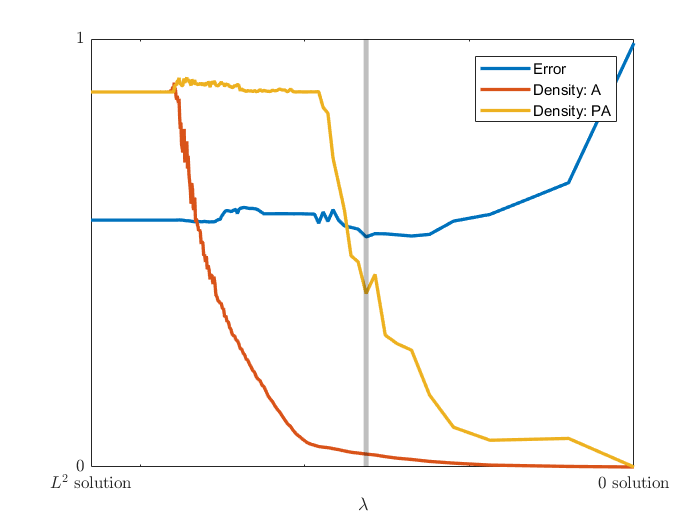
\includegraphics[width=\linewidth]{figures/lasso_ph.png}
    \caption{\Ram{This picture needs to appear later.} As the weight of the L1 penalty term increases, the Koopman operator matrix becomes more dense, and the model error decreases then levels off. This shows that there is a much sparser representation of the Koopman operator than the least-squares solution that generates a model of nearly identical accuracy.}
    \label{fig:lasso}
\end{figure}

%% FIG: Noise inherent to the system
\begin{figure}
    \centering
    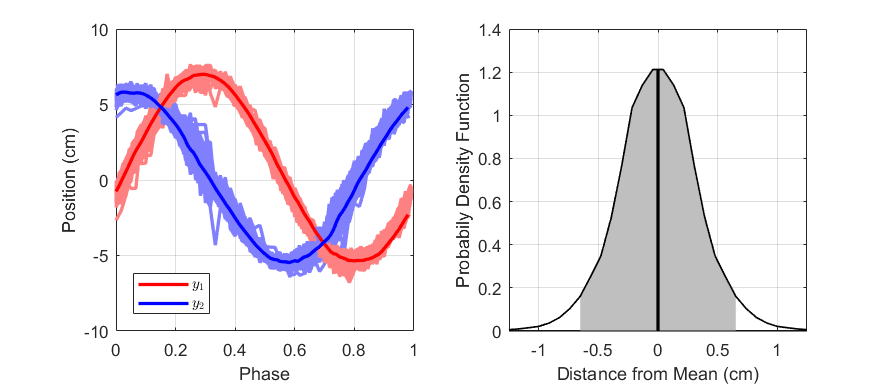
\includegraphics[width=\linewidth]{figures/noise_ph.png}
    \caption{\Dan{Need to use different colors for y1 y2. Blue and red already used to show state space vs. lifted space.}}
    \label{fig:noise}
\end{figure}


%% FIGURE: Linear vs. Koopman model predictions
\begin{figure}
    \centering
    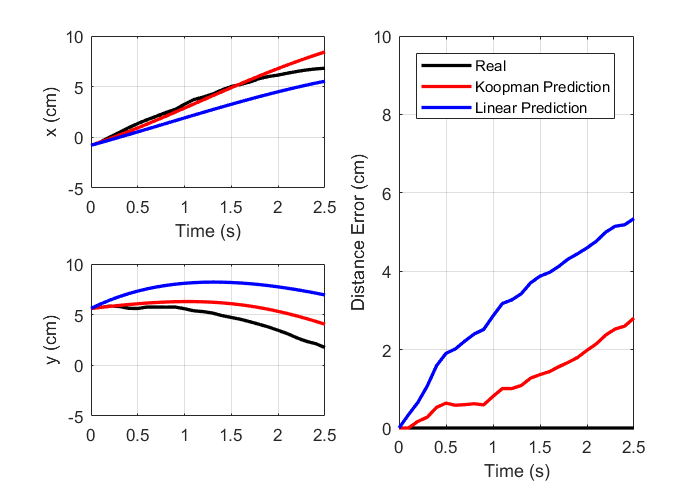
\includegraphics[width=\linewidth]{figures/predictionComparison_ph.png}
    \caption{\Dan{Placeholder for plot showing the prediction comparison between the koopman and the linear state space model.}}
    \label{fig:compare_blockM}
\end{figure}

%% FIGURE: Visual comparison of controller performance for the block M.
\begin{figure*}
    \centering
    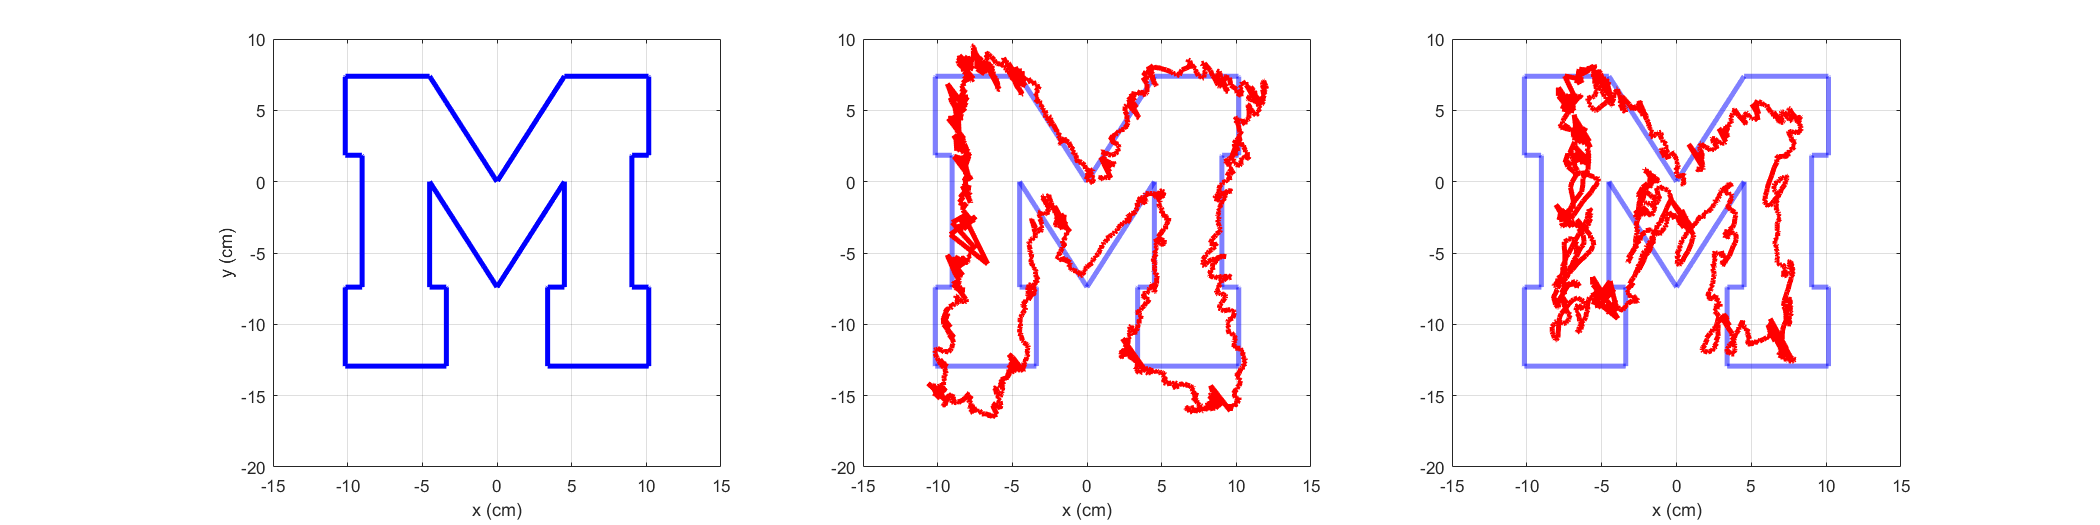
\includegraphics[width=\linewidth]{figures/compare_blockM_300s_draft.png}
    \caption{The results of each controller to performing task 1. Reference trajectory only (left). Koopman MPC (middle). Linear MPC (right). Laser dot trajectory is shown in red, the reference trajectory is shown in blue.}
    \label{fig:compare_blockM}
\end{figure*}

%% FIGURE: Visual comparison of controller performance for the pacman.
\begin{figure*}
    \centering
    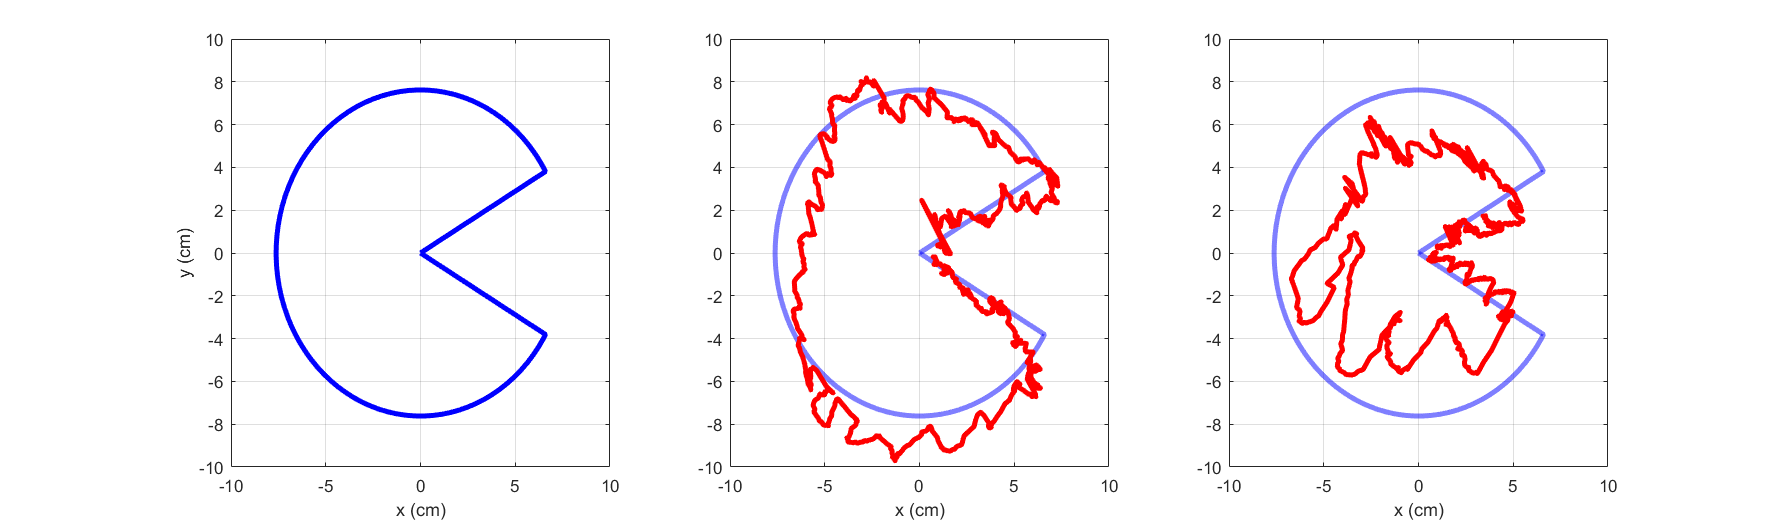
\includegraphics[width=\linewidth]{figures/compare_pacman68_90s_draft.png}
    \caption{The results of each controller to performing task 2. Reference trajectory only (left). Koopman MPC (middle). Linear MPC (right). Laser dot trajectory is shown in red, the reference trajectory is shown in blue.}
    \label{fig:compare_pacman}
\end{figure*}

%% TABLE: RMSE results table
\begin{table}[]
    \rowcolors{2}{white}{gray!25}
    \setlength\tabcolsep{5pt} % default value: 6pt
    \centering
    \caption{RMSE (cm) over all trajectory following tasks \Dan{Fill in real results later}}
    \begin{tabular}{|c|c|c|c|c|c|c|c|c|}
        \hline
        \rowcolor{white} 
        & \multicolumn{6}{c |}{\textbf{Task}} & & \textbf{Std.} \\
        \cline{2-7} \rowcolor{white}
        \multirow{-2}{*}{\textbf{Controller}} & $1$ & $2$ & $3$ & $4$ & $5$ & $6$ & \multirow{-2}{*}{\textbf{Avg.}} & \textbf{Dev.} \\
        \hline
        % RESULTS FOR ROBOT A
        Koopman MPC &  2.4  &  2.0  &  2.9  &  1.7  &  1.5  &  2.0 & 2.1 & 0.5 \\
        Linear MPC  &  5.8  &  4.0  &  6.6  &  3.9  &  2.8  &  3.5 & 4.5 & 1.5 \\
        Nonlinear MPC &  5.1  &  3.1  &  9.9  &  3.0  &  1.8  &  4.8 & 4.6 & 2.9 \\
        % Ham.-Weiner &  7.0  &  4.5  &  6.9  &  3.0  &  2.3  &  3.1 & 4.5 & 2.0 \\
        % \multirow{-5}{*}{\cellcolor{white} \rotatebox[origin=c]{90}{\textbf{Robot A}}}
        % NLARX       &  5.0  &  3.0 &  12.0  &  3.8  &  2.1  &  2.8 & 4.8 & 3.7 \\
        \hline
        % % RESULTS FOR ROBOT B
        % \cellcolor{white} & Koopman & & & & & & & & \\
        % \cellcolor{white} & Neural Net & & & & & & & & \\
        % \cellcolor{white} & State Space & & & & & & & & \\
        % \cellcolor{white} & Ham.-Weiner & & & & & & & & \\
        % \multirow{-5}{*}{\cellcolor{white} \rotatebox[origin=c]{90}{\textbf{Robot B}}}
        % & NLARX & & & & & & & & \\
        % \hline
    \end{tabular}
    \label{tab:RMSE}
\end{table}

\section{Conclusion}
\label{sec:conclusion}

% Reiteration of contribution
In this work, a data-driven modeling and control method based on Koopman operator theory was successfully applied to a soft robot.
The Koopman-based MPC controller was shown to be capable of commanding a soft robot to follow a reference trajectory better than an MPC controller based on another linear data-driven model.
% Reiterarion of why important for soft robotics
By making explicit control-oriented models of soft robots easier to construct, this method enables the rapid development of new control strategies and applications.

% Current shortcomings that should be addressed in future work (more dynamics excitement, higher dimensional systems)
While these preliminary results are promising, further work is needed to make such methods feasible for higher dimensional robotic systems.
Toward that end, this work introduced a method for promoting sparsity in matrix representations of the Koopman model.
Additional work will explore strategies for further promoting sparsity, choosing the most effective basis of observables, and building models that can account for external loading and contact forces.





% \Dan{For now this is just a list of talking points}
% Discussion of results:
% The model predictive controller using the the Koopman model outperformed the other controllers in a variety of trajectory following tasks.

% Sources of Error:
% -Model inaccuracies due to insufficient data.
% -Model inaccuracies due to Koopman truncation.
% -Poor performance of electronic pressure regulators.
% -Limited accuracy of camera based laser tracking system.

% Current Shortcomings of Method:
% -Curse of dimensionality, but sparsity could help (cite that paper)
% -Does not generalize outside of observed data, could be solved by switching controllers/hybrid models.

% Take Aways:
% -Has potential to revolutionize soft robot control by providing much more control friendly representation of dynamics.
% -Soft robots are well suited for a data-driven method because they can be observed safely under randomized control inputs.
% -This is the first time this method has been shown to be effective for controlling a real soft robotic system.

\section*{Acknowledgments}

%% Use plainnat to work nicely with natbib. 

\bibliographystyle{plainnat}
\bibliography{references}

\end{document}
